\documentclass[11pt,letterpaper,twocolumn]{article}
\usepackage{graphicx}
\usepackage{fullpage}
\usepackage{url}
\usepackage{amsmath}
\usepackage{booktabs}
\usepackage{fancyvrb}
\usepackage{subfig}
\usepackage{booktabs}
\usepackage{multicol}
\usepackage{multirow}
\usepackage{color}
\usepackage[colorlinks,backref]{hyperref}

\graphicspath{{figures/}}

%\linespread{1.5} % Need more space for figures

% Make LaTeX pack figures more tightly with the text
\renewcommand\dblfloatpagefraction{.90}
\renewcommand\dbltopfraction{.80}
\renewcommand\floatpagefraction{.90}
\renewcommand\topfraction{.80}
\renewcommand\bottomfraction{.80}
\renewcommand\textfraction{.1}

\begin{document}
\title{Quadruped Robot} % TODO: Better title
\author{Tom Most \and Davidy Baty \and Mark Jacobson}

\maketitle

\begin{figure}[b]
	\centering
		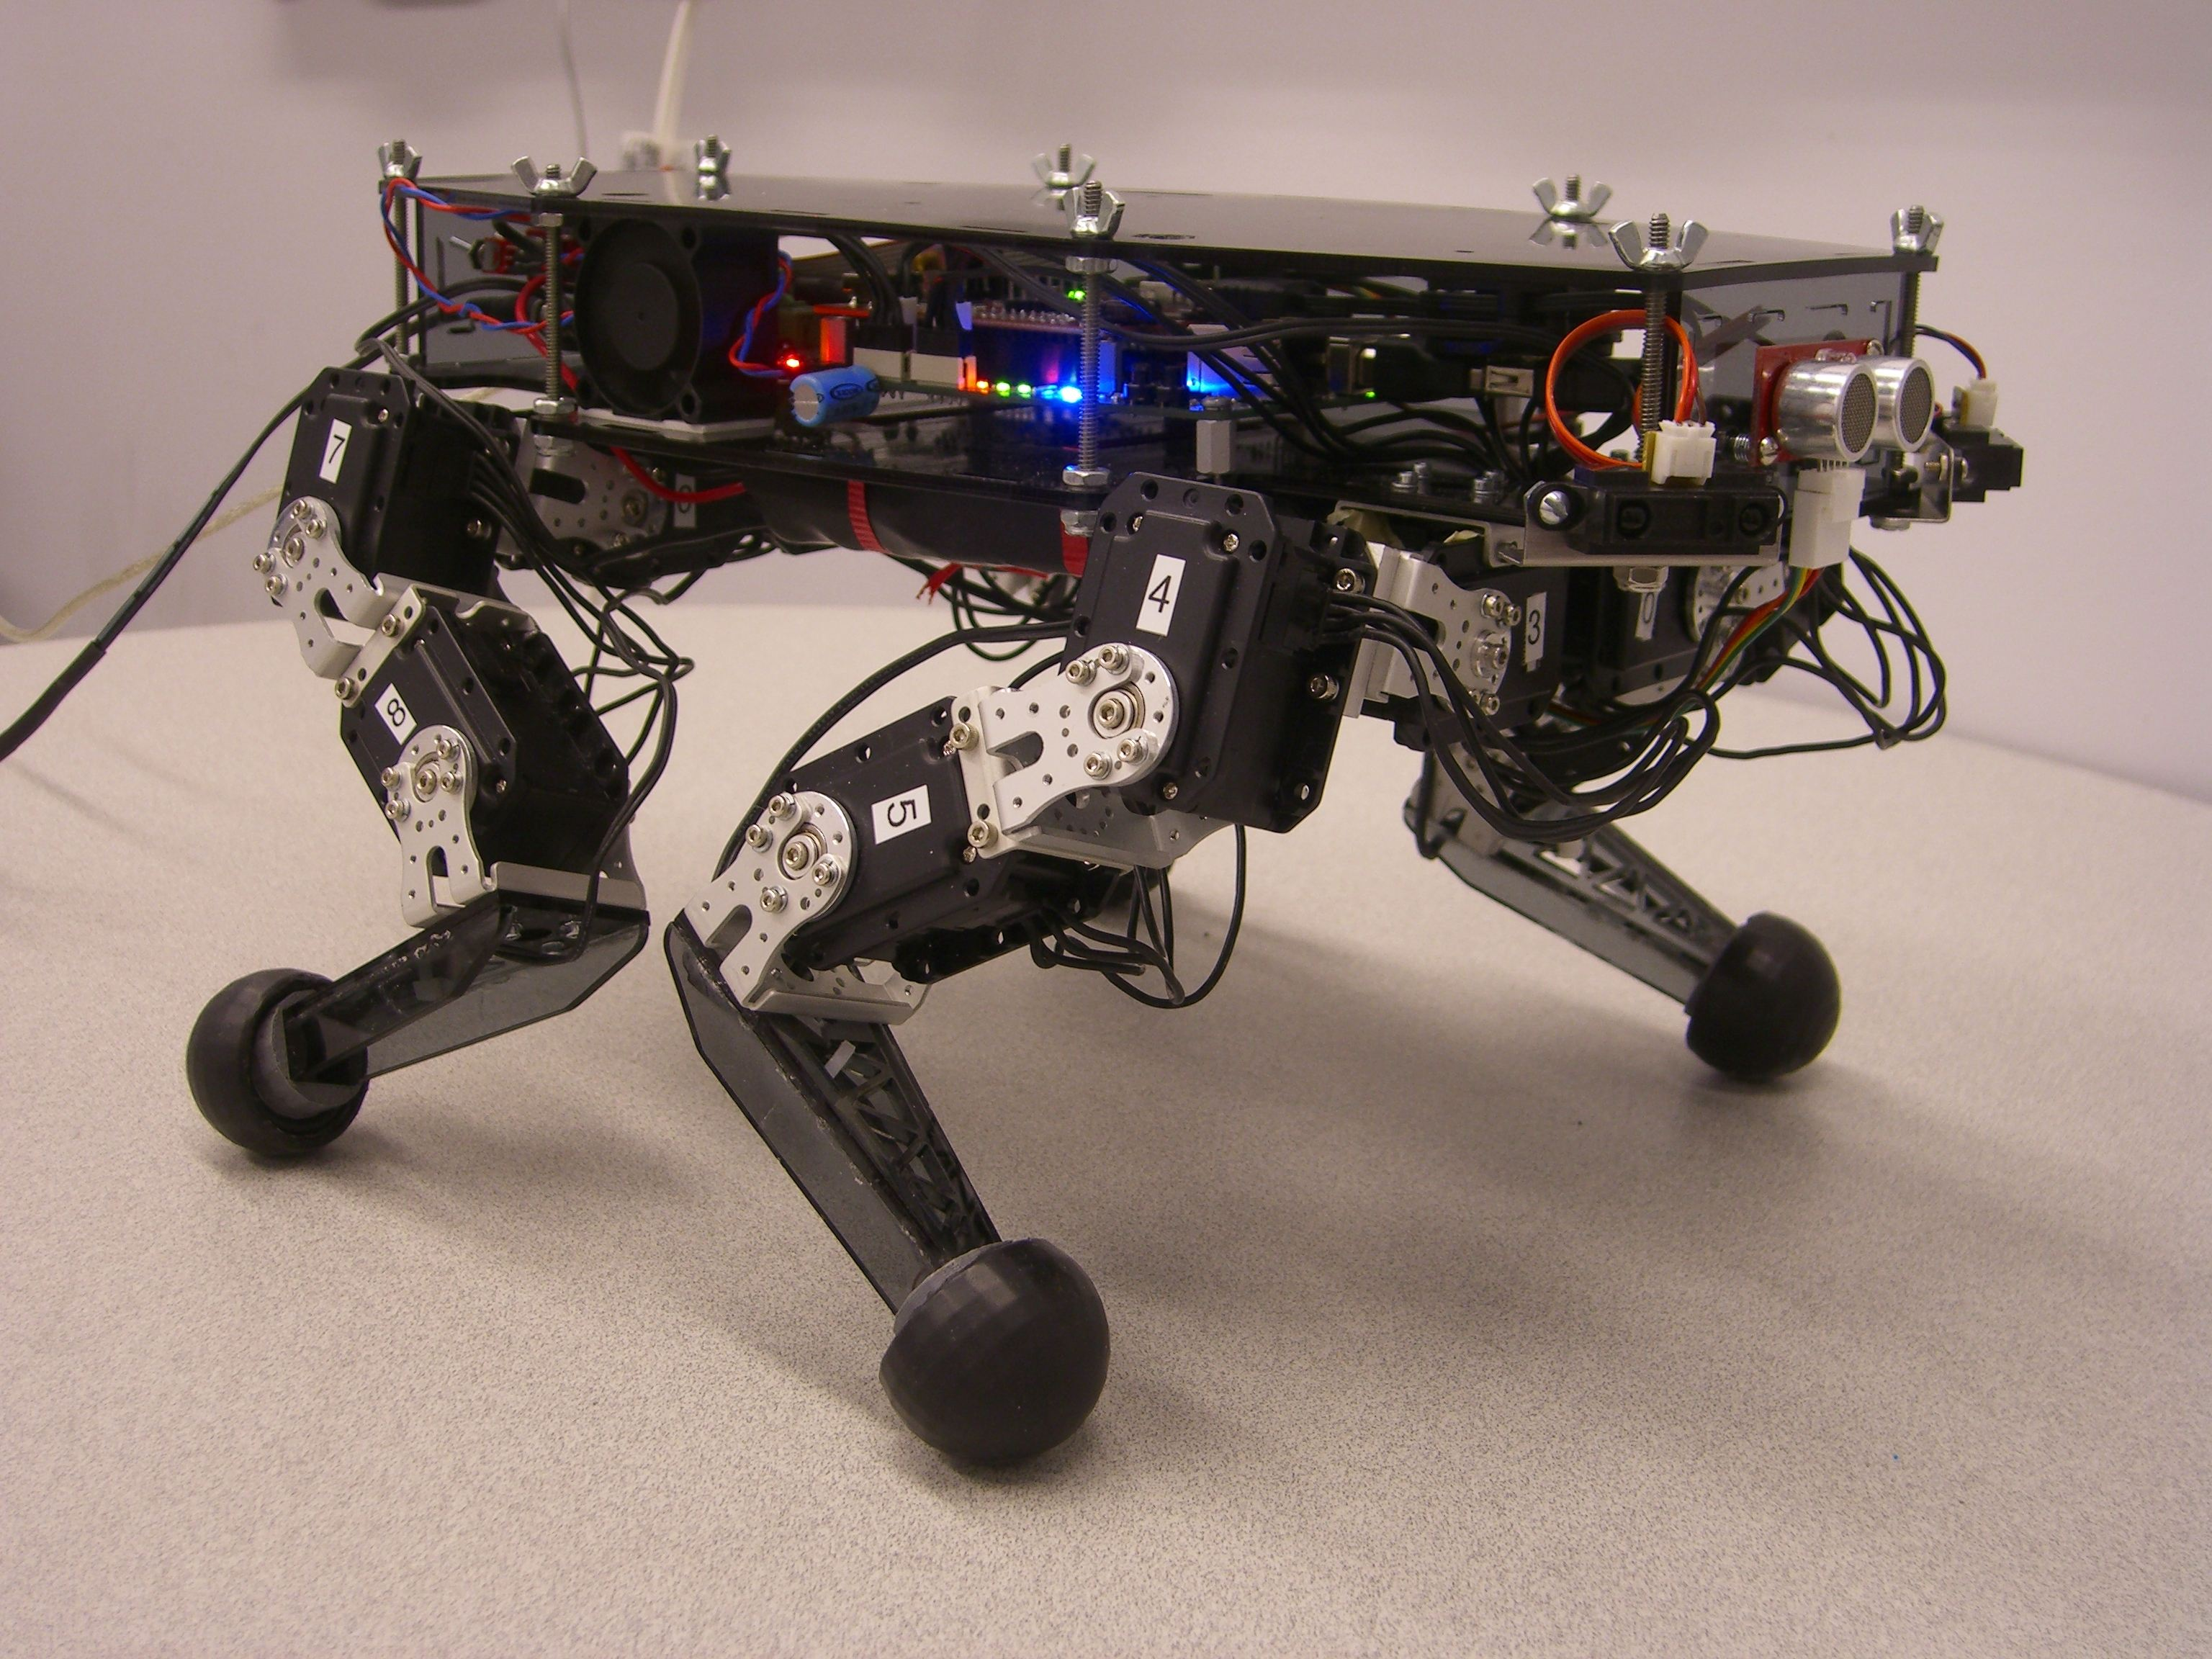
\includegraphics[width=0.5\textwidth]{cimg7445-robot.jpg}
	\caption{The completed quadruped robot.}
\end{figure}


\begin{abstract}
Foo bar baz
\end{abstract}

\section{Introduction}


Foo bar baz.

%\bibliographystyle{plain}
%\bibliography{references.bib}

\end{document}

